\documentclass[]{article}
\usepackage{lmodern}
\usepackage{amssymb,amsmath}
\usepackage{ifxetex,ifluatex}
\usepackage{fixltx2e} % provides \textsubscript
\ifnum 0\ifxetex 1\fi\ifluatex 1\fi=0 % if pdftex
  \usepackage[T1]{fontenc}
  \usepackage[utf8]{inputenc}
\else % if luatex or xelatex
  \ifxetex
    \usepackage{mathspec}
  \else
    \usepackage{fontspec}
  \fi
  \defaultfontfeatures{Ligatures=TeX,Scale=MatchLowercase}
\fi
% use upquote if available, for straight quotes in verbatim environments
\IfFileExists{upquote.sty}{\usepackage{upquote}}{}
% use microtype if available
\IfFileExists{microtype.sty}{%
\usepackage{microtype}
\UseMicrotypeSet[protrusion]{basicmath} % disable protrusion for tt fonts
}{}
\usepackage[margin=1in]{geometry}
\usepackage{hyperref}
\hypersetup{unicode=true,
            pdftitle={Rapport},
            pdfauthor={Grimaux Nicolas Sensey Valentin},
            pdfborder={0 0 0},
            breaklinks=true}
\urlstyle{same}  % don't use monospace font for urls
\usepackage{color}
\usepackage{fancyvrb}
\newcommand{\VerbBar}{|}
\newcommand{\VERB}{\Verb[commandchars=\\\{\}]}
\DefineVerbatimEnvironment{Highlighting}{Verbatim}{commandchars=\\\{\}}
% Add ',fontsize=\small' for more characters per line
\usepackage{framed}
\definecolor{shadecolor}{RGB}{248,248,248}
\newenvironment{Shaded}{\begin{snugshade}}{\end{snugshade}}
\newcommand{\AlertTok}[1]{\textcolor[rgb]{0.94,0.16,0.16}{#1}}
\newcommand{\AnnotationTok}[1]{\textcolor[rgb]{0.56,0.35,0.01}{\textbf{\textit{#1}}}}
\newcommand{\AttributeTok}[1]{\textcolor[rgb]{0.77,0.63,0.00}{#1}}
\newcommand{\BaseNTok}[1]{\textcolor[rgb]{0.00,0.00,0.81}{#1}}
\newcommand{\BuiltInTok}[1]{#1}
\newcommand{\CharTok}[1]{\textcolor[rgb]{0.31,0.60,0.02}{#1}}
\newcommand{\CommentTok}[1]{\textcolor[rgb]{0.56,0.35,0.01}{\textit{#1}}}
\newcommand{\CommentVarTok}[1]{\textcolor[rgb]{0.56,0.35,0.01}{\textbf{\textit{#1}}}}
\newcommand{\ConstantTok}[1]{\textcolor[rgb]{0.00,0.00,0.00}{#1}}
\newcommand{\ControlFlowTok}[1]{\textcolor[rgb]{0.13,0.29,0.53}{\textbf{#1}}}
\newcommand{\DataTypeTok}[1]{\textcolor[rgb]{0.13,0.29,0.53}{#1}}
\newcommand{\DecValTok}[1]{\textcolor[rgb]{0.00,0.00,0.81}{#1}}
\newcommand{\DocumentationTok}[1]{\textcolor[rgb]{0.56,0.35,0.01}{\textbf{\textit{#1}}}}
\newcommand{\ErrorTok}[1]{\textcolor[rgb]{0.64,0.00,0.00}{\textbf{#1}}}
\newcommand{\ExtensionTok}[1]{#1}
\newcommand{\FloatTok}[1]{\textcolor[rgb]{0.00,0.00,0.81}{#1}}
\newcommand{\FunctionTok}[1]{\textcolor[rgb]{0.00,0.00,0.00}{#1}}
\newcommand{\ImportTok}[1]{#1}
\newcommand{\InformationTok}[1]{\textcolor[rgb]{0.56,0.35,0.01}{\textbf{\textit{#1}}}}
\newcommand{\KeywordTok}[1]{\textcolor[rgb]{0.13,0.29,0.53}{\textbf{#1}}}
\newcommand{\NormalTok}[1]{#1}
\newcommand{\OperatorTok}[1]{\textcolor[rgb]{0.81,0.36,0.00}{\textbf{#1}}}
\newcommand{\OtherTok}[1]{\textcolor[rgb]{0.56,0.35,0.01}{#1}}
\newcommand{\PreprocessorTok}[1]{\textcolor[rgb]{0.56,0.35,0.01}{\textit{#1}}}
\newcommand{\RegionMarkerTok}[1]{#1}
\newcommand{\SpecialCharTok}[1]{\textcolor[rgb]{0.00,0.00,0.00}{#1}}
\newcommand{\SpecialStringTok}[1]{\textcolor[rgb]{0.31,0.60,0.02}{#1}}
\newcommand{\StringTok}[1]{\textcolor[rgb]{0.31,0.60,0.02}{#1}}
\newcommand{\VariableTok}[1]{\textcolor[rgb]{0.00,0.00,0.00}{#1}}
\newcommand{\VerbatimStringTok}[1]{\textcolor[rgb]{0.31,0.60,0.02}{#1}}
\newcommand{\WarningTok}[1]{\textcolor[rgb]{0.56,0.35,0.01}{\textbf{\textit{#1}}}}
\usepackage{graphicx,grffile}
\makeatletter
\def\maxwidth{\ifdim\Gin@nat@width>\linewidth\linewidth\else\Gin@nat@width\fi}
\def\maxheight{\ifdim\Gin@nat@height>\textheight\textheight\else\Gin@nat@height\fi}
\makeatother
% Scale images if necessary, so that they will not overflow the page
% margins by default, and it is still possible to overwrite the defaults
% using explicit options in \includegraphics[width, height, ...]{}
\setkeys{Gin}{width=\maxwidth,height=\maxheight,keepaspectratio}
\IfFileExists{parskip.sty}{%
\usepackage{parskip}
}{% else
\setlength{\parindent}{0pt}
\setlength{\parskip}{6pt plus 2pt minus 1pt}
}
\setlength{\emergencystretch}{3em}  % prevent overfull lines
\providecommand{\tightlist}{%
  \setlength{\itemsep}{0pt}\setlength{\parskip}{0pt}}
\setcounter{secnumdepth}{0}
% Redefines (sub)paragraphs to behave more like sections
\ifx\paragraph\undefined\else
\let\oldparagraph\paragraph
\renewcommand{\paragraph}[1]{\oldparagraph{#1}\mbox{}}
\fi
\ifx\subparagraph\undefined\else
\let\oldsubparagraph\subparagraph
\renewcommand{\subparagraph}[1]{\oldsubparagraph{#1}\mbox{}}
\fi

%%% Use protect on footnotes to avoid problems with footnotes in titles
\let\rmarkdownfootnote\footnote%
\def\footnote{\protect\rmarkdownfootnote}

%%% Change title format to be more compact
\usepackage{titling}

% Create subtitle command for use in maketitle
\providecommand{\subtitle}[1]{
  \posttitle{
    \begin{center}\large#1\end{center}
    }
}

\setlength{\droptitle}{-2em}

  \title{Rapport}
    \pretitle{\vspace{\droptitle}\centering\huge}
  \posttitle{\par}
    \author{Grimaux Nicolas Sensey Valentin}
    \preauthor{\centering\large\emph}
  \postauthor{\par}
      \predate{\centering\large\emph}
  \postdate{\par}
    \date{27/10/2019}


\begin{document}
\maketitle

{
\setcounter{tocdepth}{2}
\tableofcontents
}
\hypertarget{pruxe9sentation-des-donnuxe9es}{%
\section{Présentation des
données}\label{pruxe9sentation-des-donnuxe9es}}

\begin{figure}
\centering
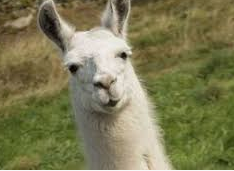
\includegraphics{../images/test.png}
\caption{coucoulol}
\end{figure}

Le travail demandé consiste à analyser un jeu de donnée concernant les
députés français. Les sources des données sont les suivantes :

\href{https://projetarcadie.com/tableaux-thematiques}{Projet arcadie}

\href{http://data.assemblee-nationale.fr/}{Données de l'Assemblée
Nationale}

Les variables et les méthodes à utiliser pour effectuer les analyses
sont libres. Le jeu de données fourni est un fichier de format
\emph{.xlsx} comprenant 4 tables :

\begin{itemize}
\tightlist
\item
  \textbf{deputestable1} : comprend 575 observations et 11 variables
  notamment les Nom, Prénom, Région, Profession et Groupe politique
  (complet) et Groupe politique(abrégé)
\item
  \textbf{deputestable2} : comprend 576 observations et 12 variables.
  Mis à part le Nom et le prénom cette table comprend les dates de
  naissance des députés, le statut des députés, les catégories de
  fonctionnaires\ldots{}
\item
  \textbf{deputestable3} : comprend 576 obersvations et 4 variables.
  Cette table récapitule l'historique parlementaire de chaque député.
\item
  \textbf{deputestable4} : comprend 573 observations et 45 variables.
  Cette table récapitule tout ce qu'il y a à savoir concernant les duels
  politiques des dernières éléctions (abstention, candidat en face du
  vainqueur, etc)
\end{itemize}

\hypertarget{travail-pruxe9paratoire}{%
\section{Travail préparatoire}\label{travail-pruxe9paratoire}}

\hypertarget{pruxe9requis}{%
\subsection{Prérequis}\label{pruxe9requis}}

Voici les librairies requises pour notre analyse. Certains librairies
nécessitent d'avoir Java correctement installé.

\begin{Shaded}
\begin{Highlighting}[]
\KeywordTok{install.packages}\NormalTok{(}\StringTok{"xlsx"}\NormalTok{)}
\KeywordTok{install.packages}\NormalTok{(}\StringTok{"readxl"}\NormalTok{)}
\KeywordTok{install.packages}\NormalTok{(}\StringTok{"questionr"}\NormalTok{)}
\KeywordTok{install.packages}\NormalTok{(}\StringTok{"ggplot2"}\NormalTok{)}
\KeywordTok{install.packages}\NormalTok{(}\StringTok{"scales"}\NormalTok{)}
\end{Highlighting}
\end{Shaded}

\begin{Shaded}
\begin{Highlighting}[]
\KeywordTok{library}\NormalTok{(scales)}
\KeywordTok{library}\NormalTok{(xlsx)}
\KeywordTok{library}\NormalTok{(questionr)}
\KeywordTok{library}\NormalTok{(readxl)}
\KeywordTok{library}\NormalTok{(ggplot2)}
\end{Highlighting}
\end{Shaded}

\hypertarget{importation-des-donnuxe9es-et-fusion-des-tables}{%
\subsection{Importation des données et fusion des
tables}\label{importation-des-donnuxe9es-et-fusion-des-tables}}

Nous allons maintenant importer les données dans RStudio. Pour cela nous
allons d'abord séparer notre fichier \emph{.xlsx} comprenant 4 tables en
4 fichiers \emph{.xlsx} comprenant chacun une table. Une fois ceci fait,
nous allons fusionner nos 4 tables.

A l'issue de la fusion la table complète ne comprenait plus que 571
individus, nous avons donc cherché à savoir pourquoi ces derniers n'ont
pas ``matchés''. Il s'agissait en fait de problèmes d'accent, de
majuscules ou de deuxième prénom. Voici les individus problématiques :

\begin{itemize}
\tightlist
\item
  Amal-Amélia Lakrafi : Dans les Table 2 et 3 elle se nomme
  ``Amal-Amélia Lakrafi'' et dans la Table 1 ``Amélia Lakrafi''.
\item
  Constance le Grip : Dans une des tables le ``le'' était écrit ``Le''.
\item
  Thierry Benoît : Présence de l'accent circonflexe dans certaines
  tables et pas dans les autres.
\item
  Patricia Miralles : Le ``e'' est accentué ou non suivant la table.
\item
  Pierre Venteau TABLE1: N'existe pas dans la table 1.
\end{itemize}

Nous allons corriger les problèmes d'accent et de second prénom avant
d'importer les données. Ce faisant, on corrige bien les problemes de
merge. Une seule personne disparait, cependant on veut la garder donc
nous rajouterons l'argument ``all.x=TRUE'' lors de la fusion.

Il y a également des problèmes avec la table 4. Elle comprend plusieurs
colonnes avec le même nom et la première ligne de la table ne comprend
pas les intitulés de colonnes. Nous allons donc la nettoyer au préalable
directement sur le fichier \emph{.xlsx}.

\begin{verbatim}
## New names:
## * `N°Panneau` -> `N°Panneau...19`
## * Sexe -> Sexe...20
## * Nom -> Nom...21
## * Prénom -> Prénom...22
## * Nuance -> Nuance...23
## * ... and 22 more problems
\end{verbatim}

Il convient également de créer une nouvelle colonne Titre dans
\textbf{deputestable1} pour pouvoir la fusionner avec les autres. Enfin,
une fois que nous avons la même variable pour toutes les tables, nous la
passons en majuscules afin d'éviter les erreurs mentionnées
précédemment. Nous obtenons donc une table unique que nous appelerons
\textbf{deputes}.

\begin{verbatim}
## [1] "On enlève les prenoms et noms en trop."
\end{verbatim}

\#Analyse

\emph{Note : A partir de maintenant, le code ne figurera plus dans le
corps du document mais sera mis en annexe}

\hypertarget{ruxe9partition-du-genre-au-sein-de-lan}{%
\subsection{Répartition du genre au sein de
l'AN}\label{ruxe9partition-du-genre-au-sein-de-lan}}

\begin{verbatim}
## 
##   F   M 
## 197 309
\end{verbatim}

\includegraphics{rapport_files/figure-latex/unnamed-chunk-8-1.pdf}

\hypertarget{ruxe9partition-des-partis-politques-au-sein-de-lassembluxe9e}{%
\subsection{Répartition des partis politques au sein de
l'assemblée}\label{ruxe9partition-des-partis-politques-au-sein-de-lassembluxe9e}}

\includegraphics{rapport_files/figure-latex/unnamed-chunk-9-1.pdf}

\begin{verbatim}
## [1] "Je voudrai faire un graphique sur la frequence de premier mandat par partie politique"
\end{verbatim}

\hypertarget{focus-sur-luxe2ge}{%
\subsection{Focus sur l'âge}\label{focus-sur-luxe2ge}}

To do : rappeler qu'on crée la colonne âge et dire que le code est en
annexe

\hypertarget{ruxe9partion-guxe9nuxe9rale-des-uxe2ges-au-sein-de-lassembluxe9e}{%
\subsubsection{Répartion générale des âges au sein de
l'assemblée}\label{ruxe9partion-guxe9nuxe9rale-des-uxe2ges-au-sein-de-lassembluxe9e}}

\includegraphics{rapport_files/figure-latex/unnamed-chunk-10-1.pdf}

\hypertarget{ruxe9partition-des-uxe2ges-par-parti-politique}{%
\subsubsection{Répartition des âges par parti
politique}\label{ruxe9partition-des-uxe2ges-par-parti-politique}}

\includegraphics{rapport_files/figure-latex/unnamed-chunk-11-1.pdf}

\hypertarget{uxe2ge-moyen-des-duxe9putuxe9s-par-parti-politique}{%
\subsubsection{Âge moyen des députés par parti
politique}\label{uxe2ge-moyen-des-duxe9putuxe9s-par-parti-politique}}

\includegraphics{rapport_files/figure-latex/unnamed-chunk-12-1.pdf}


\end{document}
